\section{experiments and results}

In this paper, we propose an effective system to estimate the presence or absence 
of a given ecology phenomenon (like green leaf plants) 
from visual contents of public-shared photographs. First, we employ the state-of-the-art 
computer vision technique to detect the target phenomenon. Then according to the visual evidence 
and the corresponding timestamp and geo-tag of each image, we adopt the likelihood model in ~\cite{ecology2012www}
aggregating the large scale, imperfect information to reconstruct the satellite maps.

In Scene classification, we also employ the current state-of-the-art algorithm, 
the Convolutional Neural Network (CNN) pre-trained on ImageNet dataset. 
The key idea behind this approach is that instead of selecting and combining hand designed features 
with limited parameters to fit each recognition task, it learns hierarchical image feature directly 
for target objects.
We fine-tune it with our 
hand-labeled dataset for each experiment case and further improve the performance illustrated below.


We study two important ecology phenomena, for each time period and location, 
wether there is snowfall and are there many plants with green leaves? We discuss the experimental setup 
and the results and evaluation below.

\subsection{Snow Case}
\subsubsection{Scene Classification}
%We are using the same hand-labeled dataset as in ~\cite{wang2013observing}.
Beyond combining visual features, 
we build CNN visual model for our snow scene classification problem 
by fine-tuning Imagenet pre-trained model with the 8000 training images labeled for snow scene~\cite{wang2013observing}. The best 
performance in ~\cite{wang2013observing} using visual features with SVM is $80.50\%$ accuracy.
On the same testing set of 2000 images, our CNN model achieves $88.06\%$ accuracy as a significant 
improvement. Details of comparison between performance of CNN model
 and other visual features are presented in Table ~\ref{tab:snow}. Therefore, we use this as our recognition model for final predictions.

Figure ~\ref{fig:PR_ROC_snow} compares classification performance of CNN with 
individual visual features and their combination in terms of an ROC curve, 
as well as a precision-recall curve in which the task is to retrieve photos containing snow.
The precision-recall curve of CNN shows that at about $50\%$ recall, precision is very near to $100\%$, 
while even at $80\%$ recall, precision is still above $90\%$. This is a nice feature because 
in many applications, it may not be necessary to correctly 
classify all images, but instead it is important to find some images that most likely contain snowy 
scene.

We now turn to present experimental results for estimating geo-temporal distributions of snowfall.

\subsubsection{Snow Prediction on Cities}
To compare with existing results in ~\cite{wang2013observing} using tag based method,
we first test how well our image-content based method can predict snowfall on daily base at a local scale, 
and in particular 
for the same four U.S. metropolitan areas, New York City, Boston, Chicago and Philadelphia. 
Table~\ref{tab:city_conf_tag_vision} 
shows some basic statistics for these 4 cities, and results of these classifiers. 
Best performance obtained when we combine 
the confidence scores of tags and visual model based on CNN. For each of the method, 
Chicago gives the highest accuracy while Philadelphia gets the lowest accuracy. 
It's reasonable considering that Chicago has the most active Flickr users per
day (94.9) while Philadelphia has the least (43.7). 

There is not a clear evidence that visual evidence is more informative in estimating snowfall 
presence. In contrast, it gets lower accuracy in all these 4 cities. But combining tag and visual 
confidence achieves considerable improvement in performance. We apply this combined model 
in the following experiments.

\subsubsection{Continental-scale Snow Prediction}
Adding visual evidence, we reconstruct Satellite maps and 
evaluate our model in continental scale. We follow the same metric in ~\cite{ecology2012www} to produce 
estimation at resolution of $1 \times 1$ degree (roughly $100 \times 100 km^2$) square and 1 map for 
every day in 2009 and 2010.

Figure ~\ref{fig:snowcurve} shows the precision and recall curve of snow prediction in 
continental-scale.
Here we limit our predictions for the bins which have photos taken at that 
time and location, we do this by keeping the bins have ground truth and photos at the same time. 
We computed our confidence scores based on tags and image-classification, then we trained 
simple decision tree to learn the correct thresholds to make final prediction. We achieve 
almost 0.5\% over the baseline (cutting the error rate by more than 20\%), the baseline in 
our case is the majority class which predicts now snow all the time. 



\begin{table}\centering
\caption{\textbf{Performance of different features for snow detection using SVMs for classification and compared with CNN model.}}
\label{tab:snow}
\tiny
\begin{tabular}{@{}lcr@{}}\toprule
Feature & Kernel & Accuracy\\\midrule
Random Baseline & --- & 50.0\%\\
Gist & RBF & 73.7\%\\
Color  & $\chi^2$ & 74.1\%\\
Tiny & RBF & 74.3\%\\
Spatial Color Moments & RBF & 76.2\%\\
Spatial pyramid LBP & RBF &\textbf{77.0\%}\\\midrule
All features  & linear & \textbf{80.5\%}\\
CNN& -& \textbf{88.06\%}\\
\bottomrule\\
\end{tabular}
\end{table}


\begin{figure}[th!]
\begin{center}
\vspace{-16pt}
\begin{tabular}{cc}
 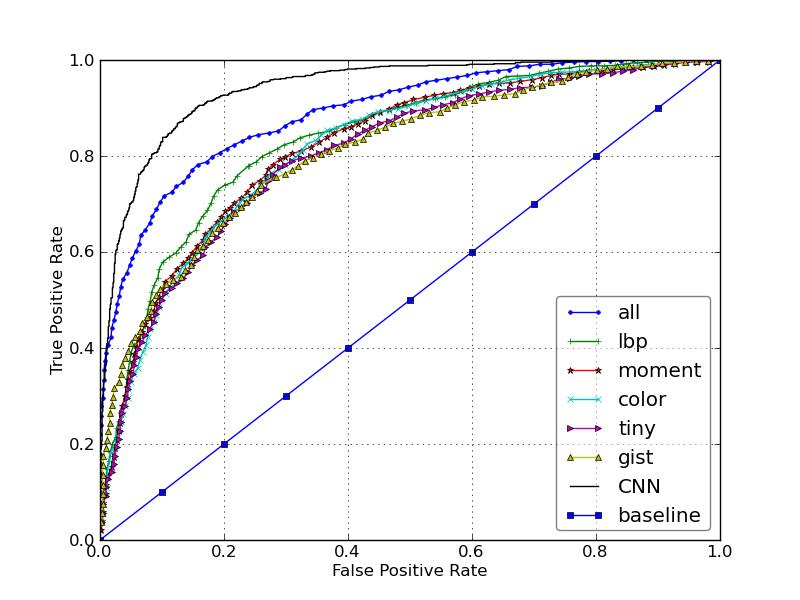
\includegraphics[width=0.2\textwidth]{figure/ROC-CNN-curves.jpg} &
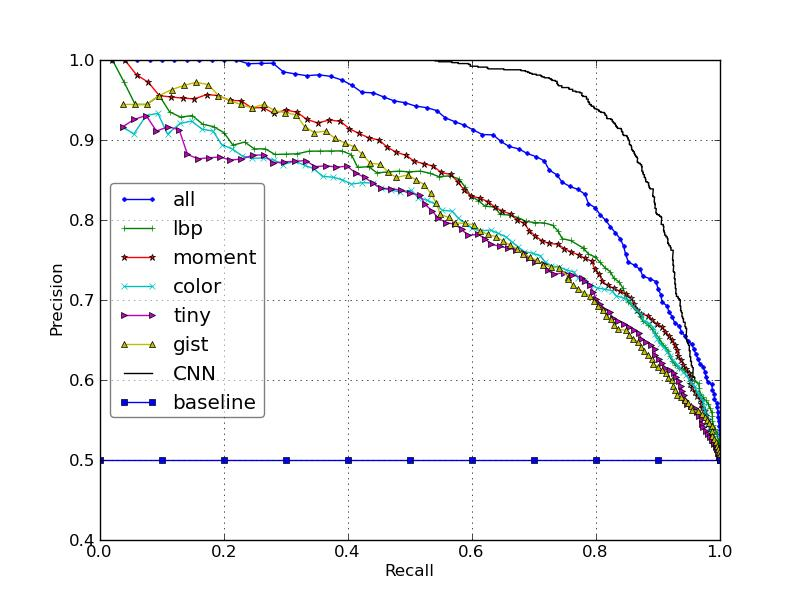
\includegraphics[width=0.2\textwidth]{figure/PR-CNN-curves.jpg} \\
\end{tabular}
\end{center}
\vspace{-8pt}
\caption{
Snow classification results for different features and combination, in terms of {\textit{(left):}} ROC curves for the task of classifying snow vs. non-snow images; and 
{\textit{(right):}} Precision-Recall curves for the task of retrieving snow images.
}
\label{fig:PR_ROC_snow}
\end{figure}


\begin{table}\centering
\caption {\textbf{Selected basic statistics during 2007 to 2010 for the 4 cities and results of the likelihood model using tags and vision evidence.}}
\label{tab:city_conf_tag_vision} 
\tiny
\begin{tabular}{@{}ccccccc@{}}\toprule
City 
& \multicolumn{1}{p{0.2cm}}{\centering naive\\baseline} 
& \multicolumn{1}{p{0.8cm}}{\centering active\\user/day} 
& \multicolumn{1}{p{0.3cm}}{\centering snow\\days} 
&  \multicolumn{1}{p{0.8cm}}{\centering tag\\confidence} 
&  \multicolumn{1}{p{0.7cm}}{\centering vision\\conf} 
& \multicolumn{1}{p{1.4cm}}{\centering tag conf \&\\vision conf} 
\\\midrule
{NYC} & 85.00\% & 65.6 & 185 &90.42\%&90.29\% &92.34\%\\
{Chicago} &72.80\% & 94.9 & 418 &94.12\% &93.16\% &95.08\%  \\
{Boston} & 75.60\%& 59.7 & 373 &89.18\%&85.21\% & 91.23\% \\
{Philly} & 80.50\% & 43.7 & 280 & 89.19\% &85.09\% & 89.19\%  \\
\bottomrule
\end{tabular}
%\vspace{-12pt}
\end{table}

\begin{figure}
\begin{center}
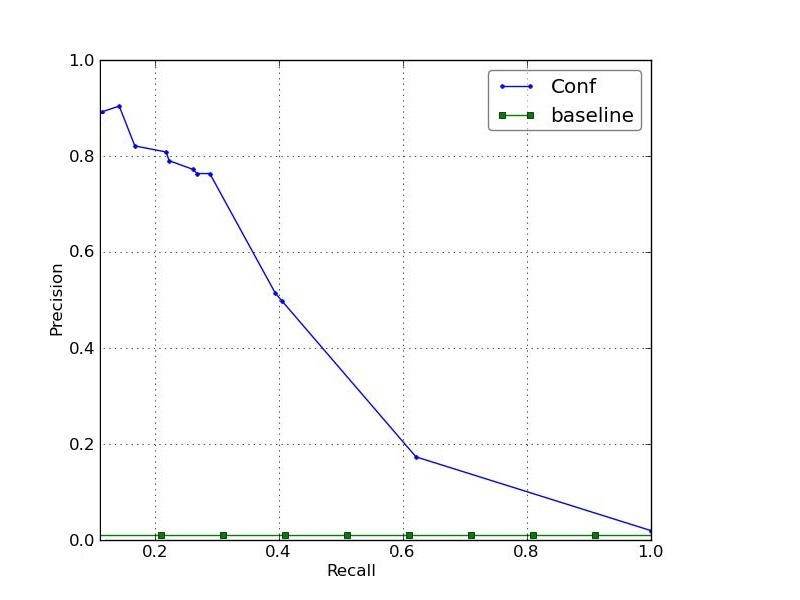
\includegraphics[width=0.2\textwidth,clip,trim=0.4in 0 0.8in 0]{figure/PR-snow.jpg}
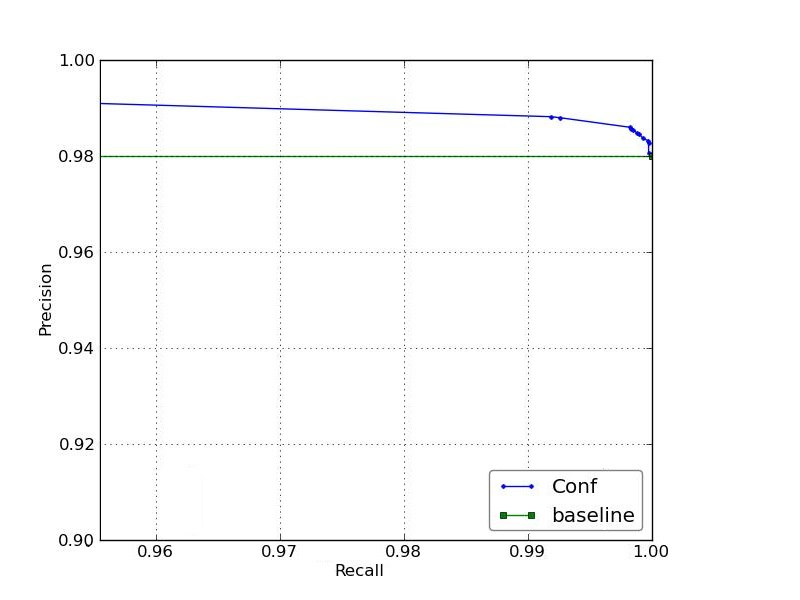
\includegraphics[width=0.2\textwidth,clip,trim=0.4in 0 0.8in 0]{figure/PR-nonsnow.jpg}
\end{center}
\vspace{-12pt}
\caption{Precision and recall curve of snow prediction (left) and nonsnow (right) in continental scale.}
\label{fig:snowcurve}
\vspace{-12pt}
\end{figure}























\subsection{Vegetation Case}
Vegetation coverage is a more stable phenomenon, so we study this case in every 16 days period instead of daily base.
Unlike snow scene that 
tag feature is very discriminative, according 
to ~\cite{ecology2012www}, textual tag of greenery is highly misleading. 
Terms like ``tree'' or even ``leaf'' are not necessarily 
indicating green color, but terms like ``green'' or 
``yellow'' could be used to describe a wild set of objects outside of vegetation. Moreover, while vegetation is 
such a common natural scene appears in most of the outdoor images, it is very unlikely people would include it in their textual tags 
to describe the image. In this case, from a huge number of images contain greenery shared online, only a very small portion of them 
actually provides related textual tags. On the other hand, we believe visual feature can be very descriptive and exclusively 
describe vegetation with green leaves.



\subsubsection{Dataset}
We build a data set with over 10000 Flickr images taken before 2009, and are composed by images with "forest" and "summer" like tags 
and also random images without any tag preference. These images are hand labeled with categories 
\textit{"Outdoor Greenery","Outdoor non-Greenery","Indoor","Other-modified"},and \textit{"Not available"}.

Finally, we build a positive set with images in category \textit{"Outdoor Greenery"} and a negative set 
with images in categories \textit{"Outdoor non-Greenery"} and \textit{"Indoor"}. To learn a image classification model, 
we build a training set with 4000 images and a testing set with 1900 images. 
In training and testing set, there are equal number of positive and negative samples.
To show the diversity of our Flickr image dataset, in figure ~\ref{fig:dataset}
we present a random sample of images in our vegetation dataset labeled as positive and negative.

In continental-scale prediction, we only look at images on Flickr.com in year 2007 to 2010, with no tag limitation. 
We filter out the photos with too unreasonable timestamps such as the taken time and uploading time is exactly the same.
We only use images with high precision geotag according to the image metadata. And we still process the 
satellite ground truth the same way as in ~\cite{ecology2012www}.



\subsubsection{Scene Classification}
We hand-labeled a separate dataset for greenery scene.
Compare to snow scene recognition,
vegetation has the signature green color that the  
biologists are very interested in during exactly which time period they are green. 
Thus it's very important 
to find out when it turns from yellow to green and when does it turns back to yellow.
The leaves of plants also have distinctive visual texture. 
Thus, visual features capture both color and texture information are our best choice.
So we employ color SIFT feature to analyze the local gradient distribution. 
And we also extract color GIST feature to describe texture feature and global context. 

\xhdr{Color SIFT histogram.}
We extract dense SIFT feature ~\cite{lowe1999object} on each of the RGB color plane, and concatenate them to 
build color SIFT feature. The dense SIFT feature is extracted from every 2 pixels by 2 pixels bin, 
with a step size of 5 pixels. In this way, we achieve representative key points and reasonable 
computation complex. 

From training data set, We build 2000 dimensional centers of color SIFT feature 
using K-means clustering. With these centers, a 2000 dimensional histogram is built 
from all the key points of each image.

\xhdr{Color GIST.} Similarly, we also extract GIST features on RGB color channel respectively.
\fxnote{From now on to the end of this paragraph, 
it's the same as our workshop paper. Could you help me to give a shorter global
description?}
GIST feature capture coarse texture
and scene layout by applying a Gabor filter bank followed by
down-sampling ~\cite{oliva2001modeling}. Our variant produces a
1536-dimensional vector and operates on color planes. Scaling
images to have square aspect ratios before computing GIST improved
classification results significantly ~\cite{douze2009evaluation}.

By concatenating color SIFT histogram and color GIST feature, 
a model is trained and tested with SVM using RBF kernel. It achieves accuracy of $85.90\%$ 
though CNN still gives a higher performance of $88.00\%$. We present detail performance in Table 
~\ref{tab:veg_img_classifier}.


%Compare to snow scene, vegetation has its strong and probably ``unique'' color and texture to be described in traditional visual 
%features, while it does not make such a difference to CNN as a data driven model. Combining color SIFT and color GIST features yields a 
%compelling prediction accuracy of $85.90\%$ though CNN still gives a higher performance of $88.00\%$. We present detail performance in Table 
%~\ref{tab:veg_img_classifier}.

\subsubsection{Vegetation Coverage over Time and Space}
We consider North America area as in snow experiments. From images in 2007 and 2008, 
we learn the prior probability of a place being covered by vegetation at any given 16-days period is $P(green) = 75.16\%$. 
For any user taken photos from a place covered by greenery at a given time, the probability of the photos contain greenery scene is 
$p = P(u|green) = 27.18\%$. On 
the other hand, there is only a small chance $q = P(u|\overline{green}) = 3.03\%$ to see a user uploading images with greenery in a place 
not covered by enough vegetation according to satellite observation. Since residence enjoy meadow around their house and it is unlikely not 
to see any plants wherever people would go, there is a considerable chance to see green scene in photos, but when there are enough users 
uploading images, we will still be able to distinguish the actual green and non-green area with the likelihood model.

While the satellite has ground truth for $87594$ bins in North America, our method predicts our method predicts $61602$ bins ($70.3\%$
 in quantity). Moreover, about $20\%$ of satellite ground truth locate in north Canada where the ecology system 
is stable and very little human-environment interaction happens. Moreover, our data is from users in social media. 
So our prediction focus on more populated locations or places people like to visit such as natural scenery.

For evaluation purpose, we only evaluate the time and location both Flickr and Satellite have data in North America. The overall accuracy 
of our method is $93.2\%$ comparing to the $86.6\%$ majority baseline. 
The precision of green bins is $98.8\%$ and the precision of non-green bins is $68.2\%$. Recall of green bins is $93.3\%$
 and recall of non-green bins is $92.5\%$. We tested the performance of using only tags to make vegetation coverage prediction 
~\cite{ecology2012www}. The performance shows tag
feature is not going to improve the result of using visual evidence. Figure ~\ref{fig:curvevege} shows the precision 
and recall curve of vegetation prediction in continental-scale.

Generally, almost all the false negative error is due to the sparseness of data. 
While not enough images are collected at certain location during some time, 
there is either no green image found or green images are too few compare to 
the quantity of non-green images. On the other hand, false positive error is rare 
(less than $1\%$) and complex. We found most images in the false positive bins are 
actually green vegetation images. ( here we need some more explanation) In figure ~\ref{fig:falseposi}, 
we show some examples of images in false positive bins. 


\subsubsection{Performance at single place over time}
For each single location, we can find out when exactly did the leaves turn yellow as well as when
did the leaves turn back to green. 
Figure ~\ref{fig:placeinbar} shows vegetation coverage of 6 places over 2009 and 2010. 
Prediction results on top usually have more data available than ground truth on the bottom. 
And we can see the ground truth is likely missing at the time when the leaves change color. 



\subsubsection{Single time over places}

Sample maps are presented in figure ~\ref{fig:map}. These maps are visualization of the performance
in North America.
We use public sharing Flickr images that are more likely taken from more populated or more popular locations. 
The satellite ground truth, instead, is limited to cloud coverage and other sensor precision issue.





\begin{figure}[th]
{\tiny{
\begin{center}
\begin{tabular}{@{}c@{\,\,\,}c@{\,\,\,}c@{\,\,\,}c@{\,\,\,}c@{\,\,\,}}
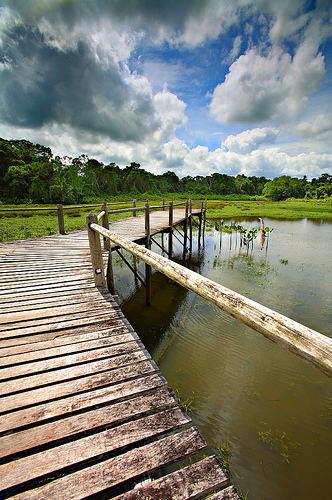
\includegraphics[width=0.06\textwidth, height=0.35in]{imggrid/datasetposi/6.jpg} &
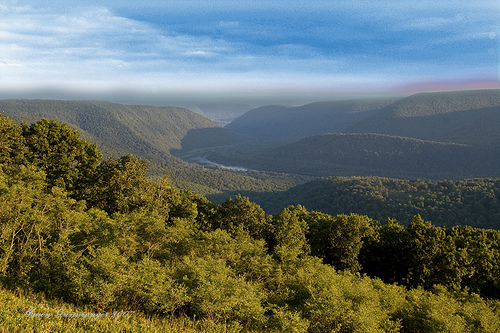
\includegraphics[width=0.06\textwidth, height=0.35in]{imggrid/datasetposi/7.jpg} &
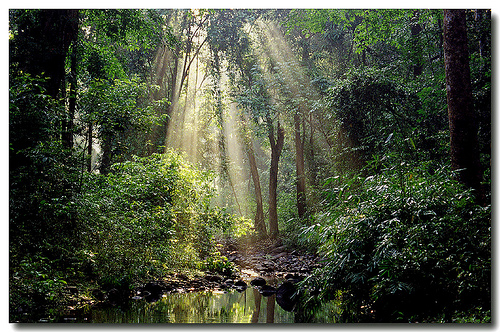
\includegraphics[width=0.06\textwidth, height=0.35in]{imggrid/datasetposi/8.jpg} &
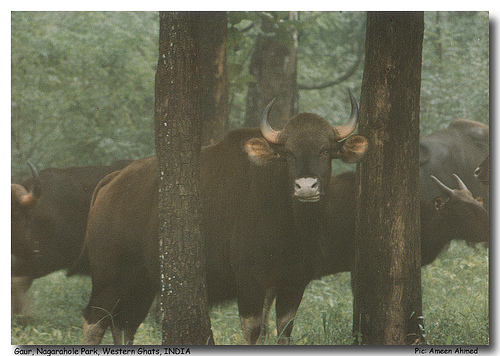
\includegraphics[width=0.06\textwidth, height=0.35in]{imggrid/datasetposi/9.jpg} &
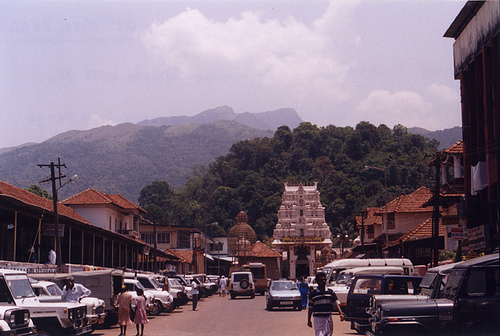
\includegraphics[width=0.06\textwidth, height=0.35in]{imggrid/datasetposi/10.jpg} \\
\multicolumn{5}{c}{(a) Random positive images in vegetation dataset} \\ 
\\[1pt]
\hline
\\[1pt]
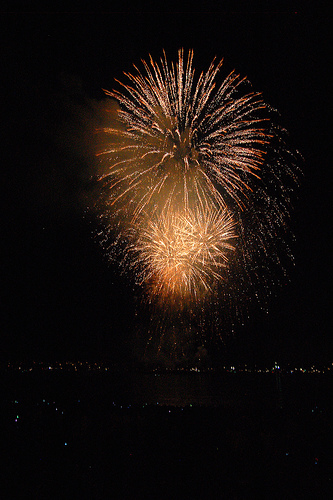
\includegraphics[width=0.06\textwidth, height=0.35in]{imggrid/datasetnega/6.jpg} &
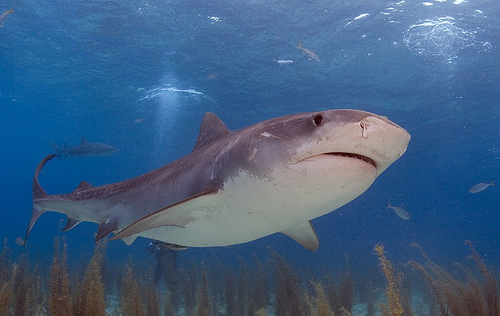
\includegraphics[width=0.06\textwidth, height=0.35in]{imggrid/datasetnega/7.jpg} &
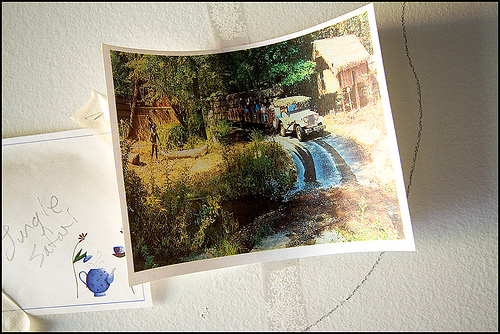
\includegraphics[width=0.06\textwidth, height=0.35in]{imggrid/datasetnega/8.jpg} &
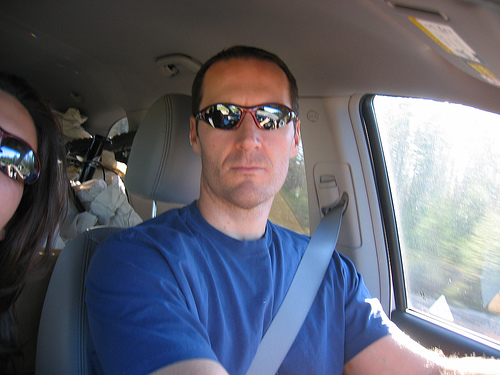
\includegraphics[width=0.06\textwidth, height=0.35in]{imggrid/datasetnega/9.jpg} &
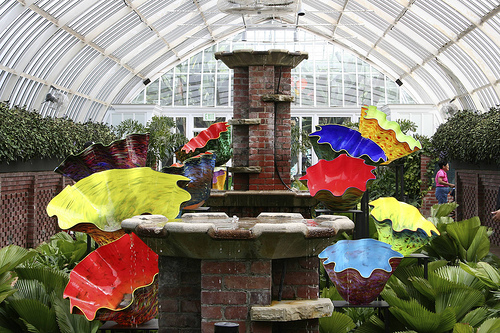
\includegraphics[width=0.06\textwidth, height=0.35in]{imggrid/datasetnega/10.jpg} \\
\multicolumn{5}{c}{(b) Random negative images in vegetation dataset} \\
\end{tabular}
\end{center}
}}
\vspace{-6pt}
\caption{Random images from our hand-labeled dataset. Public sharing images are various in quality, contents, illumination and view angle.
Negative images like winter trees without leaves, or indoor images capturing a photo of forest are more confusing.}
\label{fig:dataset}
\end{figure}

\begin{table}\centering
\caption {\textbf{Results for our visual models for vegetation.}}
\label{tab:veg_img_classifier} 
\tiny
\begin{tabular}{@{}cr@{}}\toprule
Visual feature &  Accuracy\\\midrule
Random Baseline & 50.00\%\\
Color SIFT & 78.10\%\\
Color GIST & 82.58\% \\
SIFT and GIST& 85.9\% \\
CNN\% &  88.0\%\\
\bottomrule
\end{tabular}
\end{table}

\begin{figure}
\begin{center}
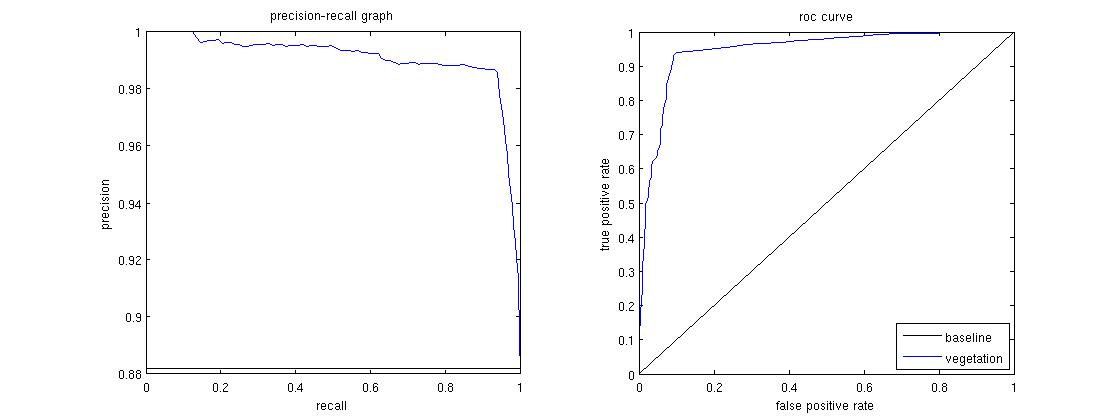
\includegraphics[width=0.45\textwidth]{figure/curvevege.jpg}
\end{center}
%}}
\vspace{-6pt}
\addvspace{2mm}
\caption{Precision and recall curve of vegetation prediction in continental scale.}
\label{fig:curvevege}
\vspace{-6pt}
\end{figure}
\addvspace{5mm}

\begin{figure}[th]
{\tiny{
\begin{center}
\begin{tabular}{@{}c@{\,\,\,}c@{\,\,\,}c@{\,\,\,}c@{\,\,\,}c@{\,\,\,}}
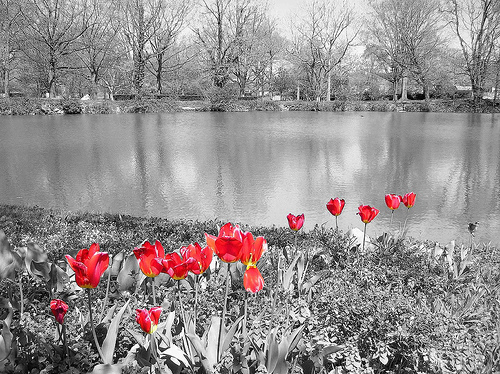
\includegraphics[width=0.06\textwidth, height=0.35in]{imggrid/falseposi/6.jpg} &
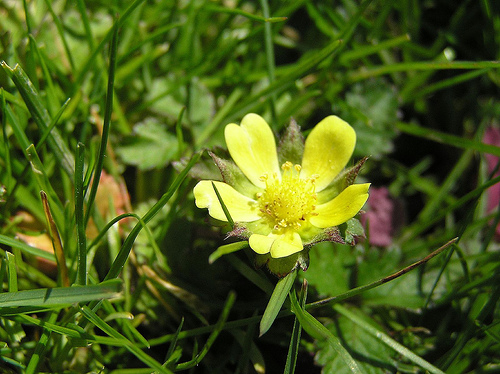
\includegraphics[width=0.06\textwidth, height=0.35in]{imggrid/falseposi/7.jpg} &
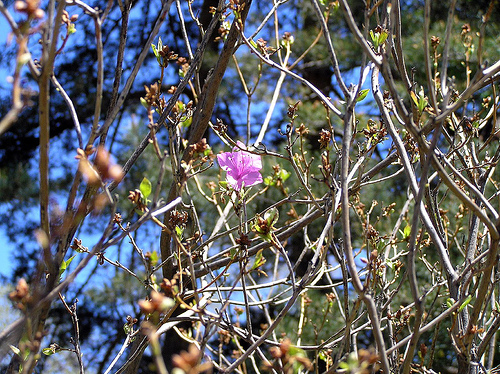
\includegraphics[width=0.06\textwidth, height=0.35in]{imggrid/falseposi/8.jpg} &
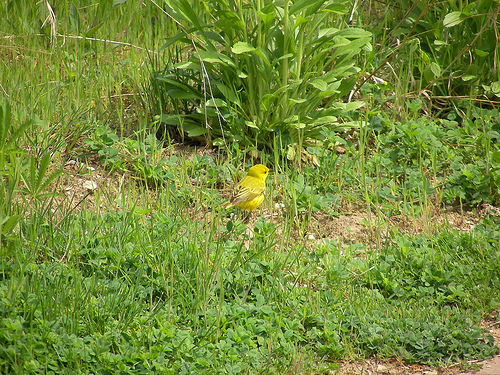
\includegraphics[width=0.06\textwidth, height=0.35in]{imggrid/falseposi/9.jpg} &
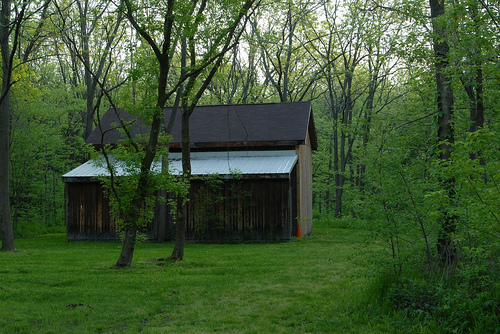
\includegraphics[width=0.06\textwidth, height=0.35in]{imggrid/falseposi/10.jpg} \\
%\multicolumn{5}{c}{(a) Random positive images in vegetation dataset} \\ 
\\[-6pt]
\hline
\\[-6pt]
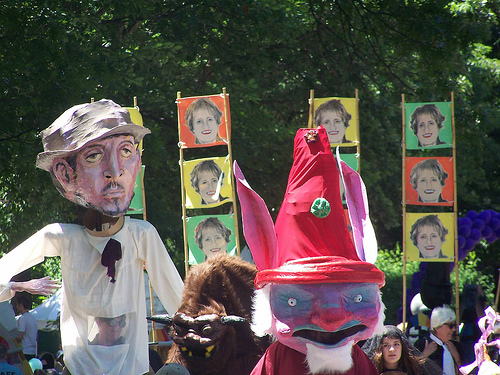
\includegraphics[width=0.06\textwidth, height=0.35in]{imggrid/falseposi/16.jpg} &
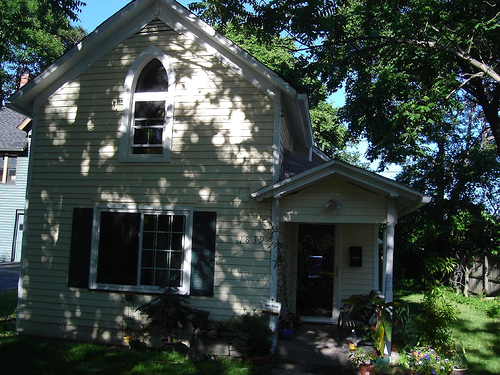
\includegraphics[width=0.06\textwidth, height=0.35in]{imggrid/falseposi/17.jpg} &
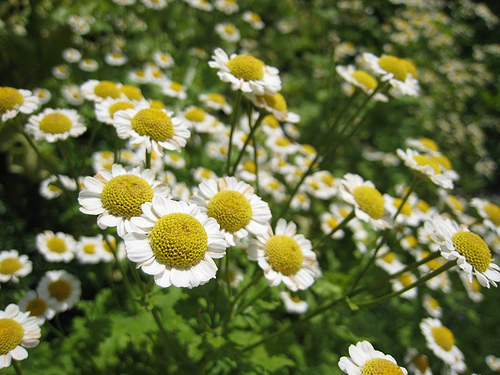
\includegraphics[width=0.06\textwidth, height=0.35in]{imggrid/falseposi/18.jpg} &
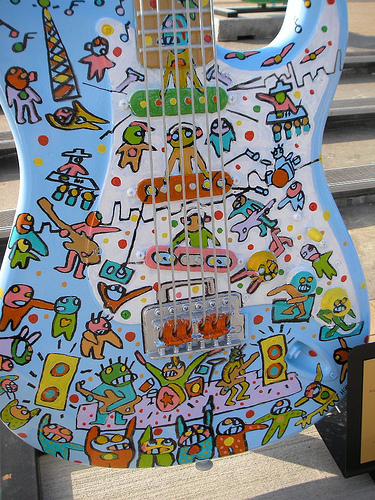
\includegraphics[width=0.06\textwidth, height=0.35in]{imggrid/falseposi/19.jpg} &
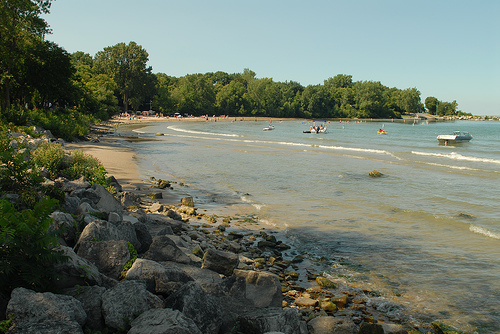
\includegraphics[width=0.06\textwidth, height=0.35in]{imggrid/falseposi/20.jpg} \\
%\multicolumn{5}{c}{(b) Random negative images in vegetation dataset} \\
\end{tabular}
\end{center}
}}
\vspace{-6pt}
\caption{In vegetation detection over North America in 2009 and 2010, among all false positive bins, there are 47 images that are predicted as greenery. And these images are the reason these bins are predicted as green. Here are some random selected examples of the green images.}
\label{fig:falseposi}
\vspace{-6pt}
\end{figure}

% bar plot of 2 places
\begin{figure}
%{\tiny{
\begin{center}
\begin{tabular}{ccc}
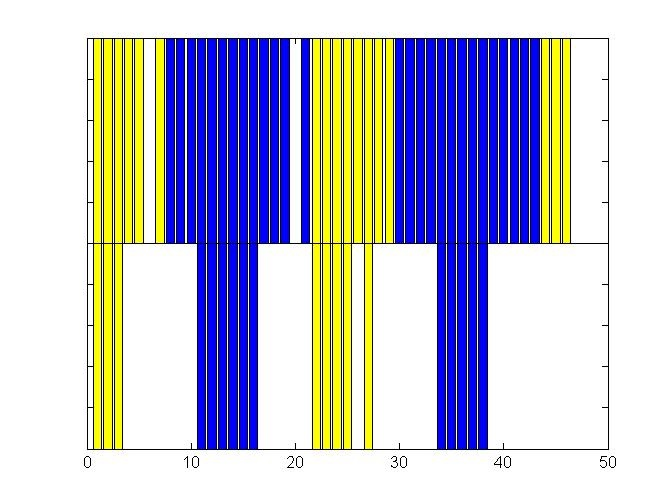
\includegraphics[width=0.14\textwidth]{bar/8560.jpg} &
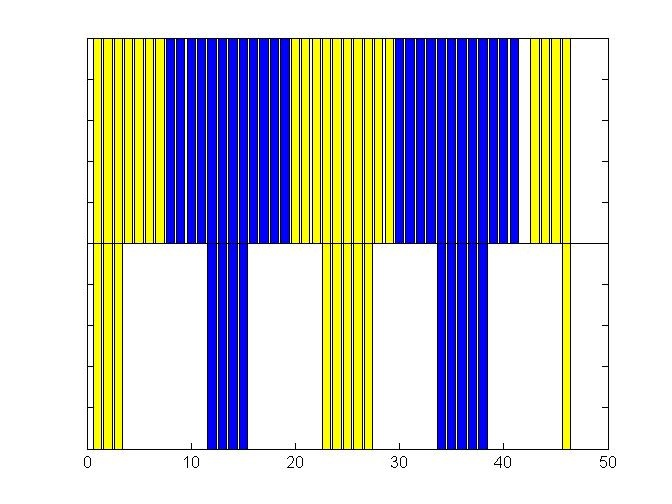
\includegraphics[width=0.14\textwidth]{bar/8561.jpg} &
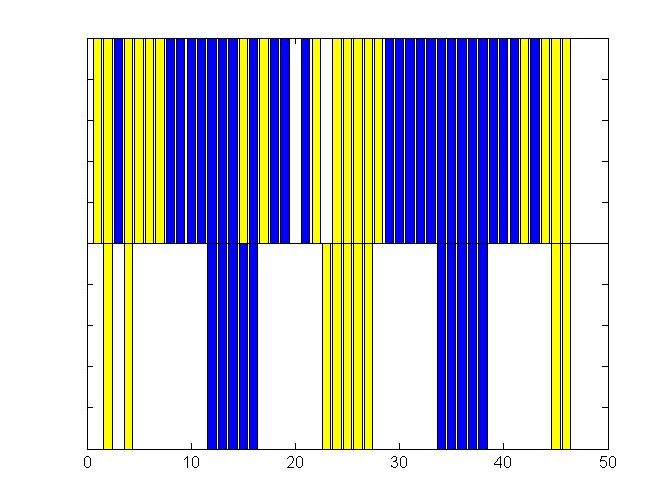
\includegraphics[width=0.14\textwidth]{bar/8881.jpg} \\
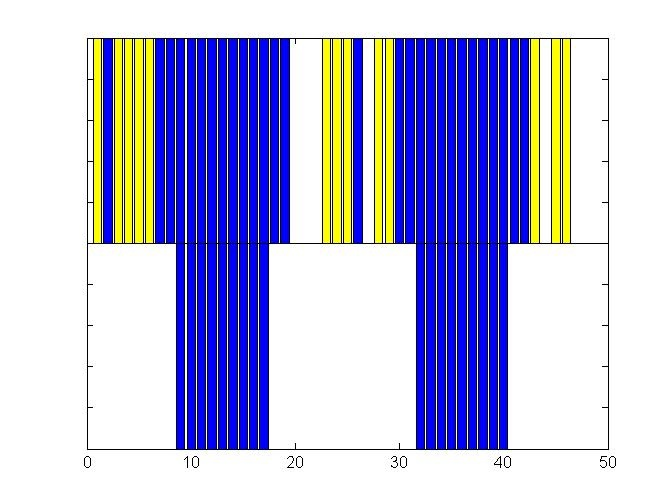
\includegraphics[width=0.14\textwidth]{bar/8911.jpg} &
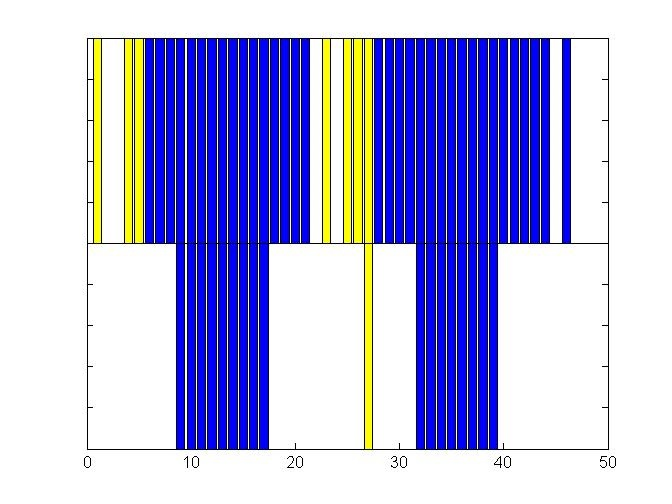
\includegraphics[width=0.14\textwidth]{bar/9705.jpg} &
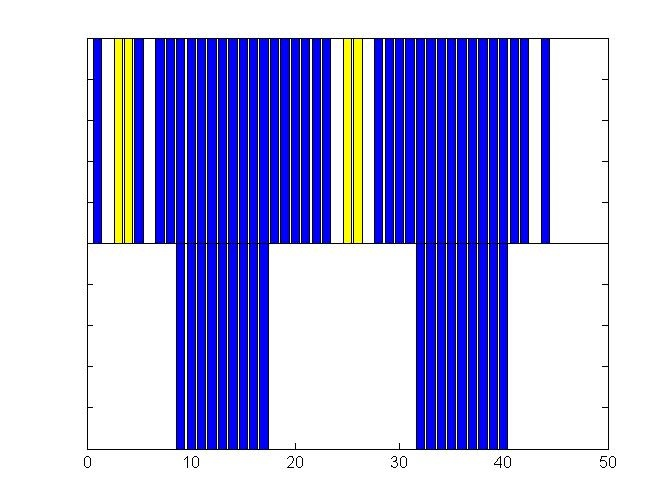
\includegraphics[width=0.14\textwidth]{bar/10816.jpg} \\
%(a) & (b)\\
\\
\end{tabular}
\end{center}
%}}
\vspace{-24pt}
\caption{Yellow bars show non-greenery at that time. Blue bars represent greenery. Prediction results on top shows 6 random places comparing to satellite ground truth. The ground truth on the bottom tends to disappear when leaves are turning yellow or green.}
\label{fig:placeinbar}
\vspace{-12pt}
\end{figure}

\begin{figure}
%{\tiny{
\begin{center}
\begin{tabular}{cccc}
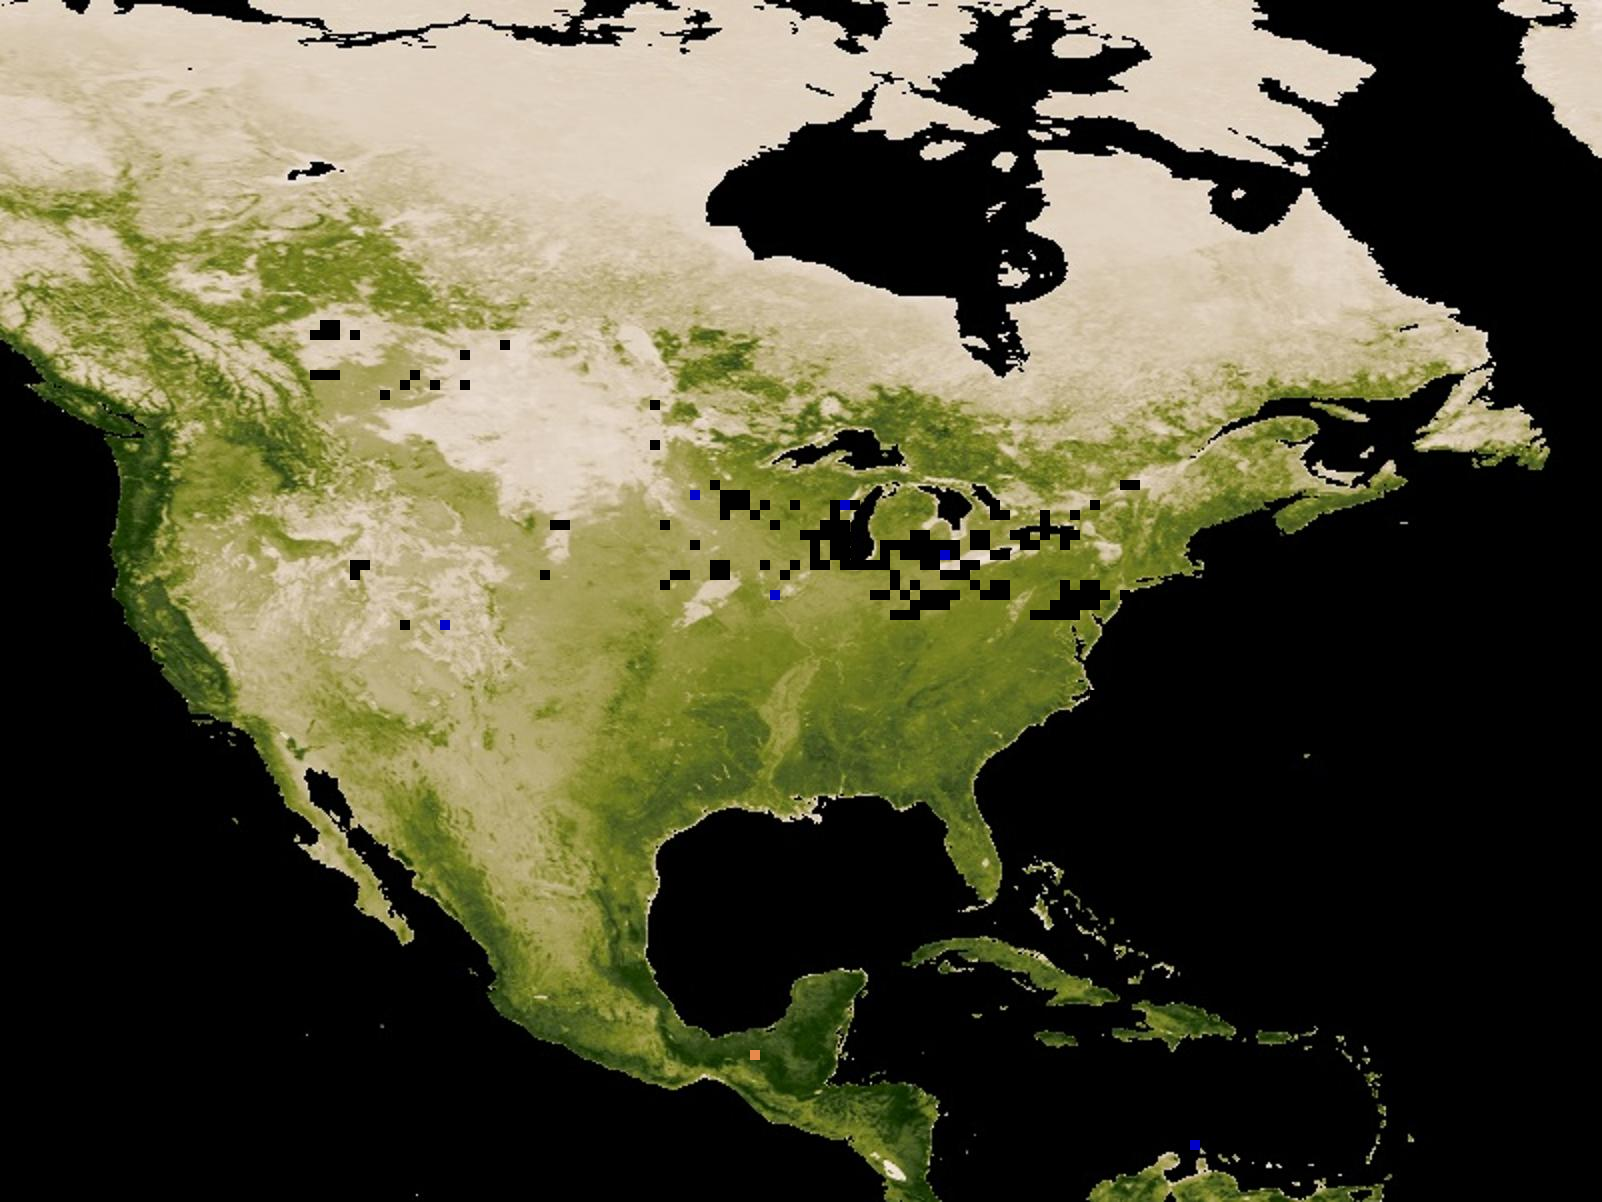
\includegraphics[width=0.10\textwidth]{map/72.png} &
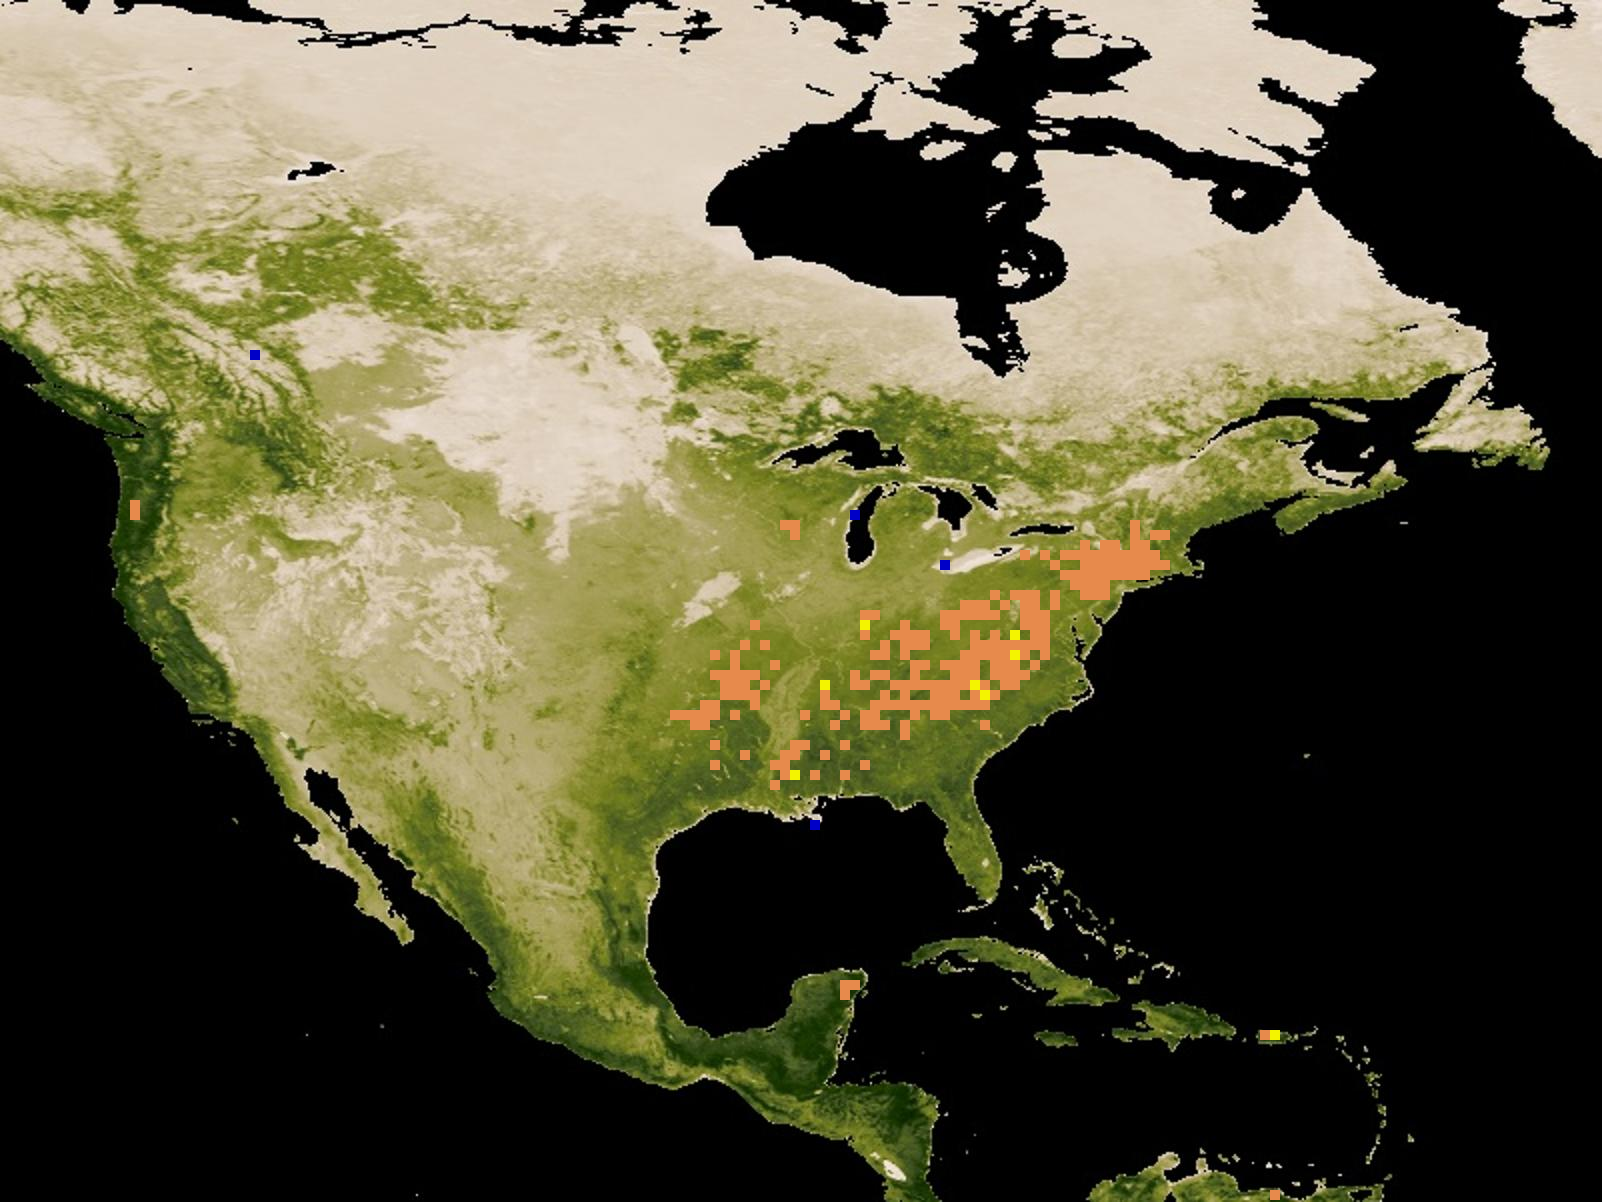
\includegraphics[width=0.10\textwidth]{map/77.png} &
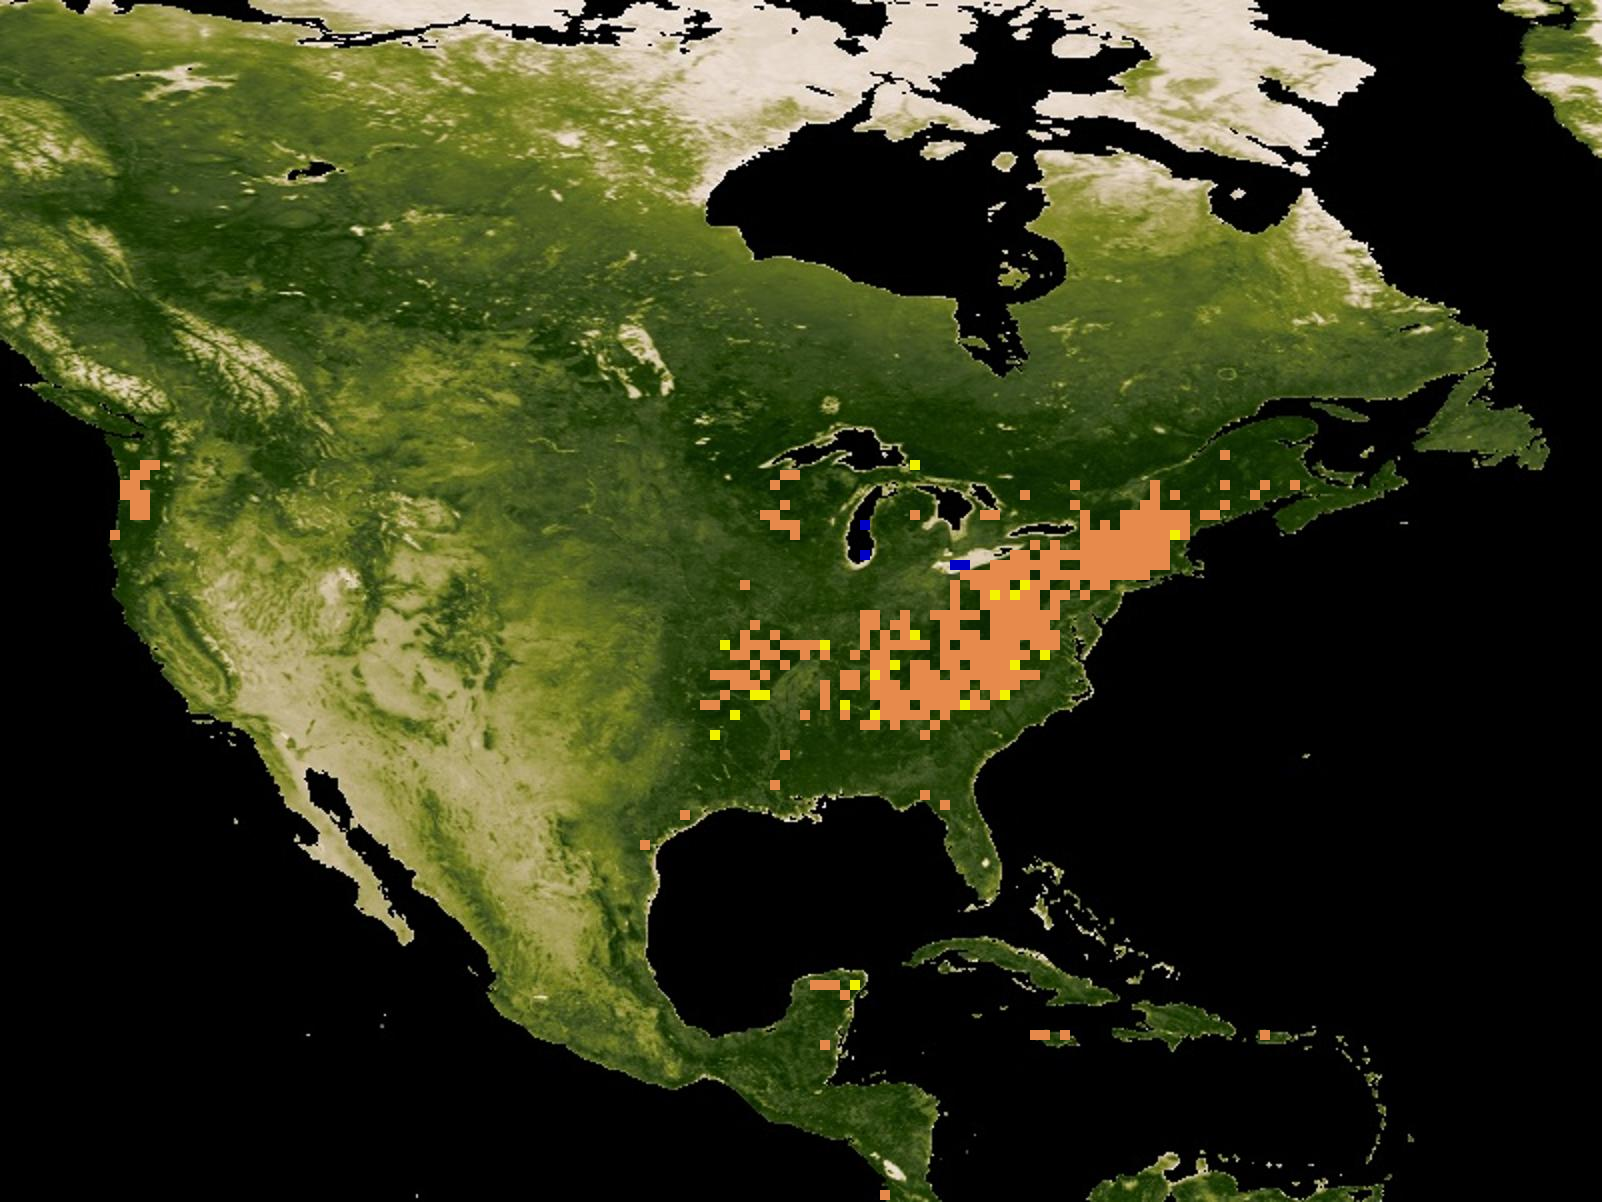
\includegraphics[width=0.10\textwidth]{map/78.png} &
%\includegraphics[width=0.5\textwidth,height=1.4in,clip,trim=0 0.5in 0in 0.6in]{plots/chicago_noaa_vs_prediction_prev_3.png} 
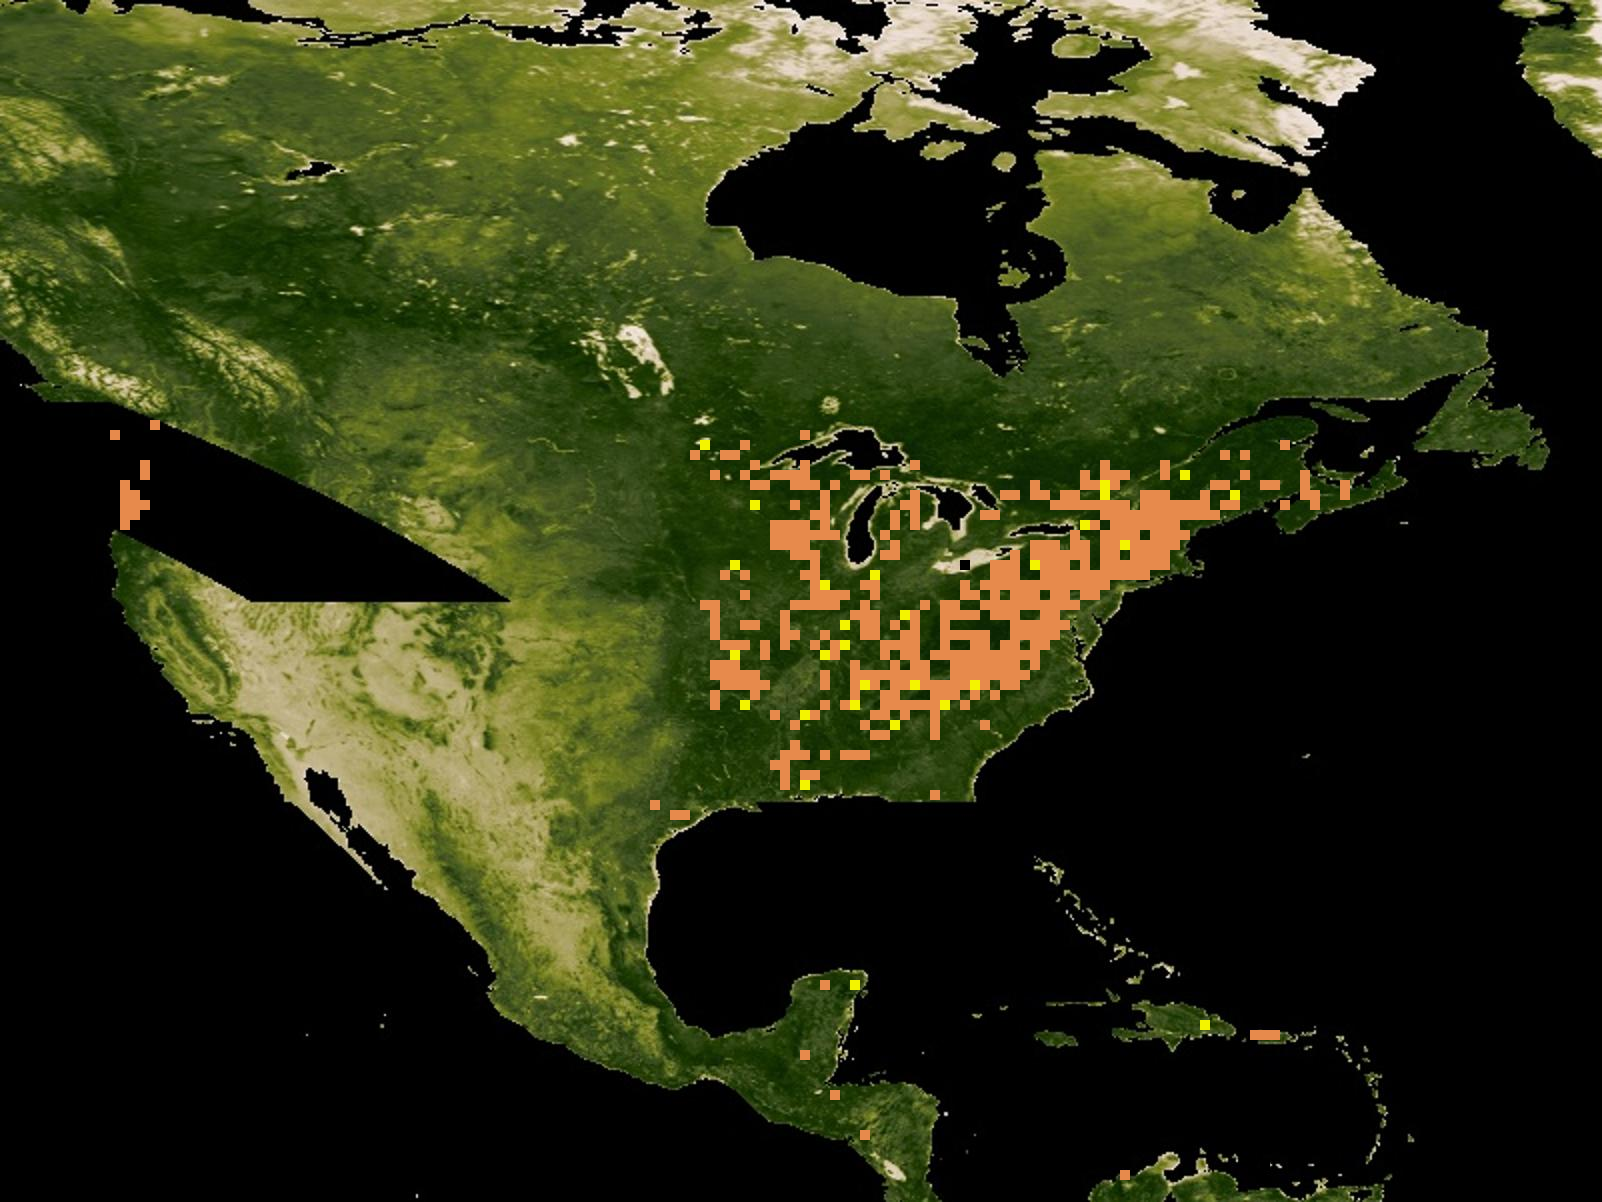
\includegraphics[width=0.10\textwidth]{map/79.png}  \\
Mar, 6th&May, 25th&Jun, 10th&Jun, 26th\\
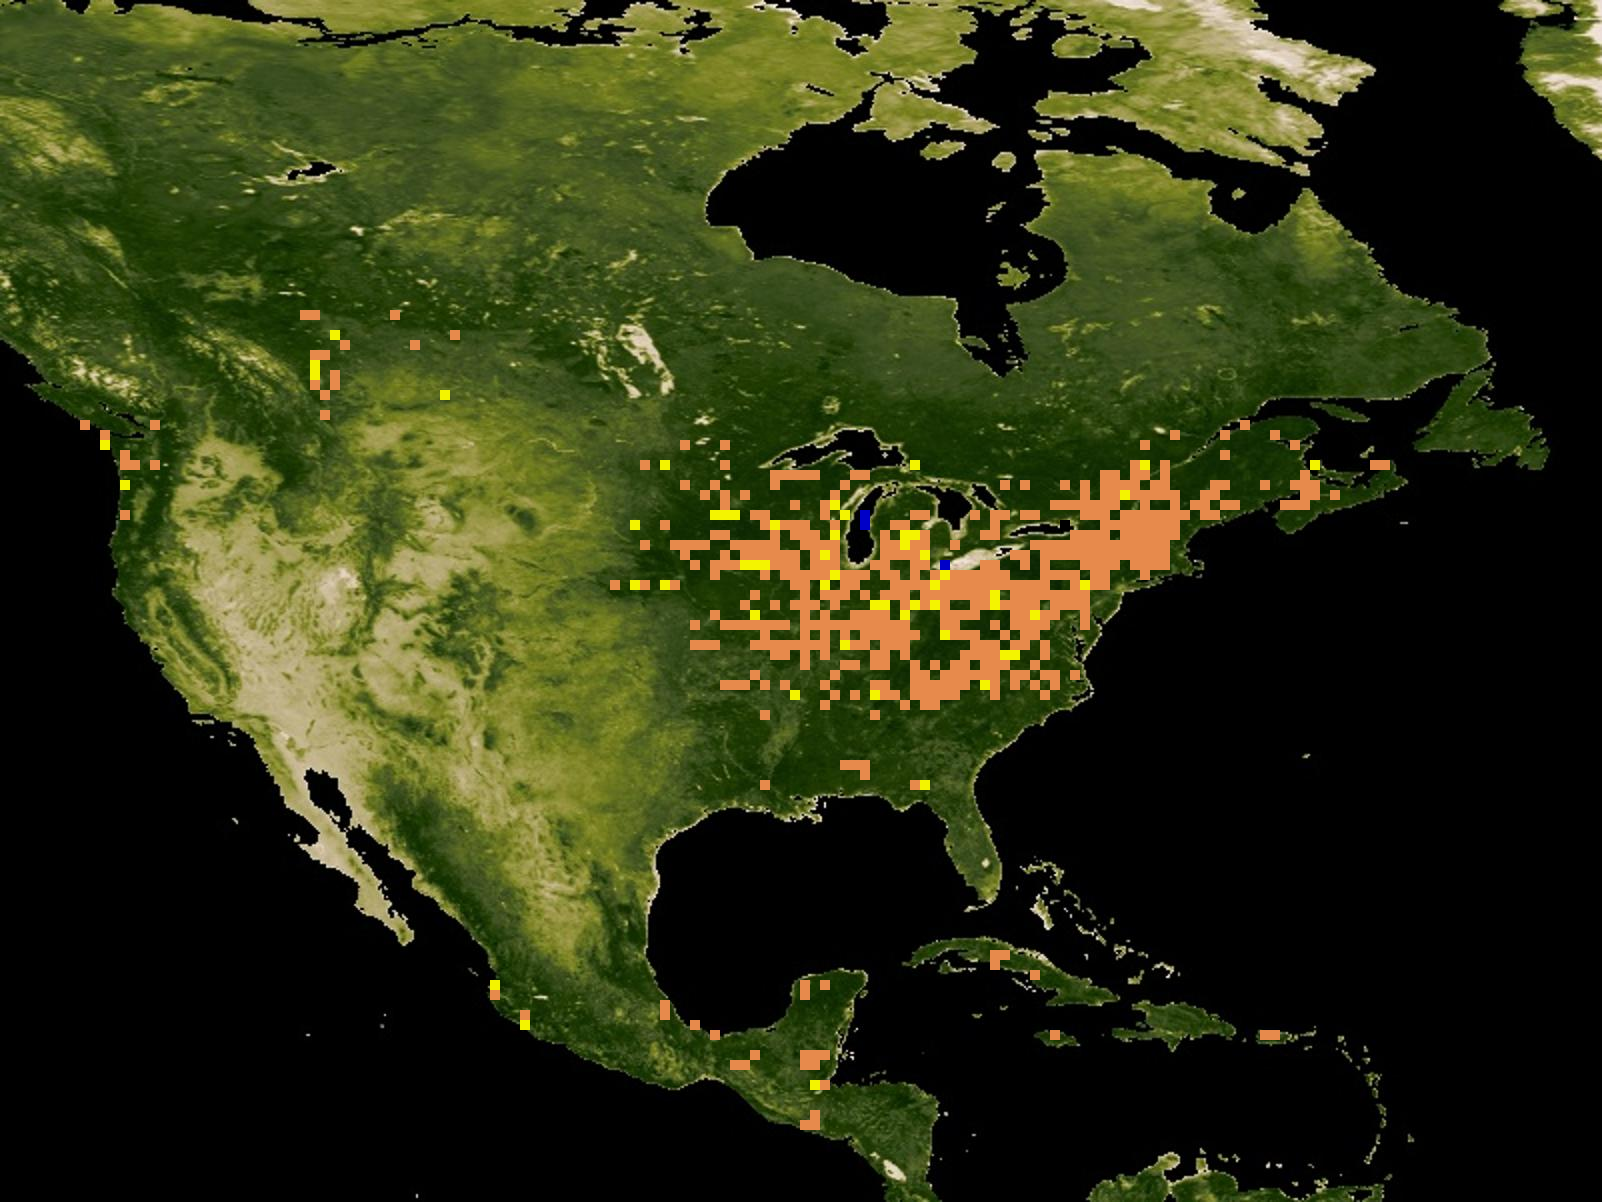
\includegraphics[width=0.10\textwidth]{map/82.png} &
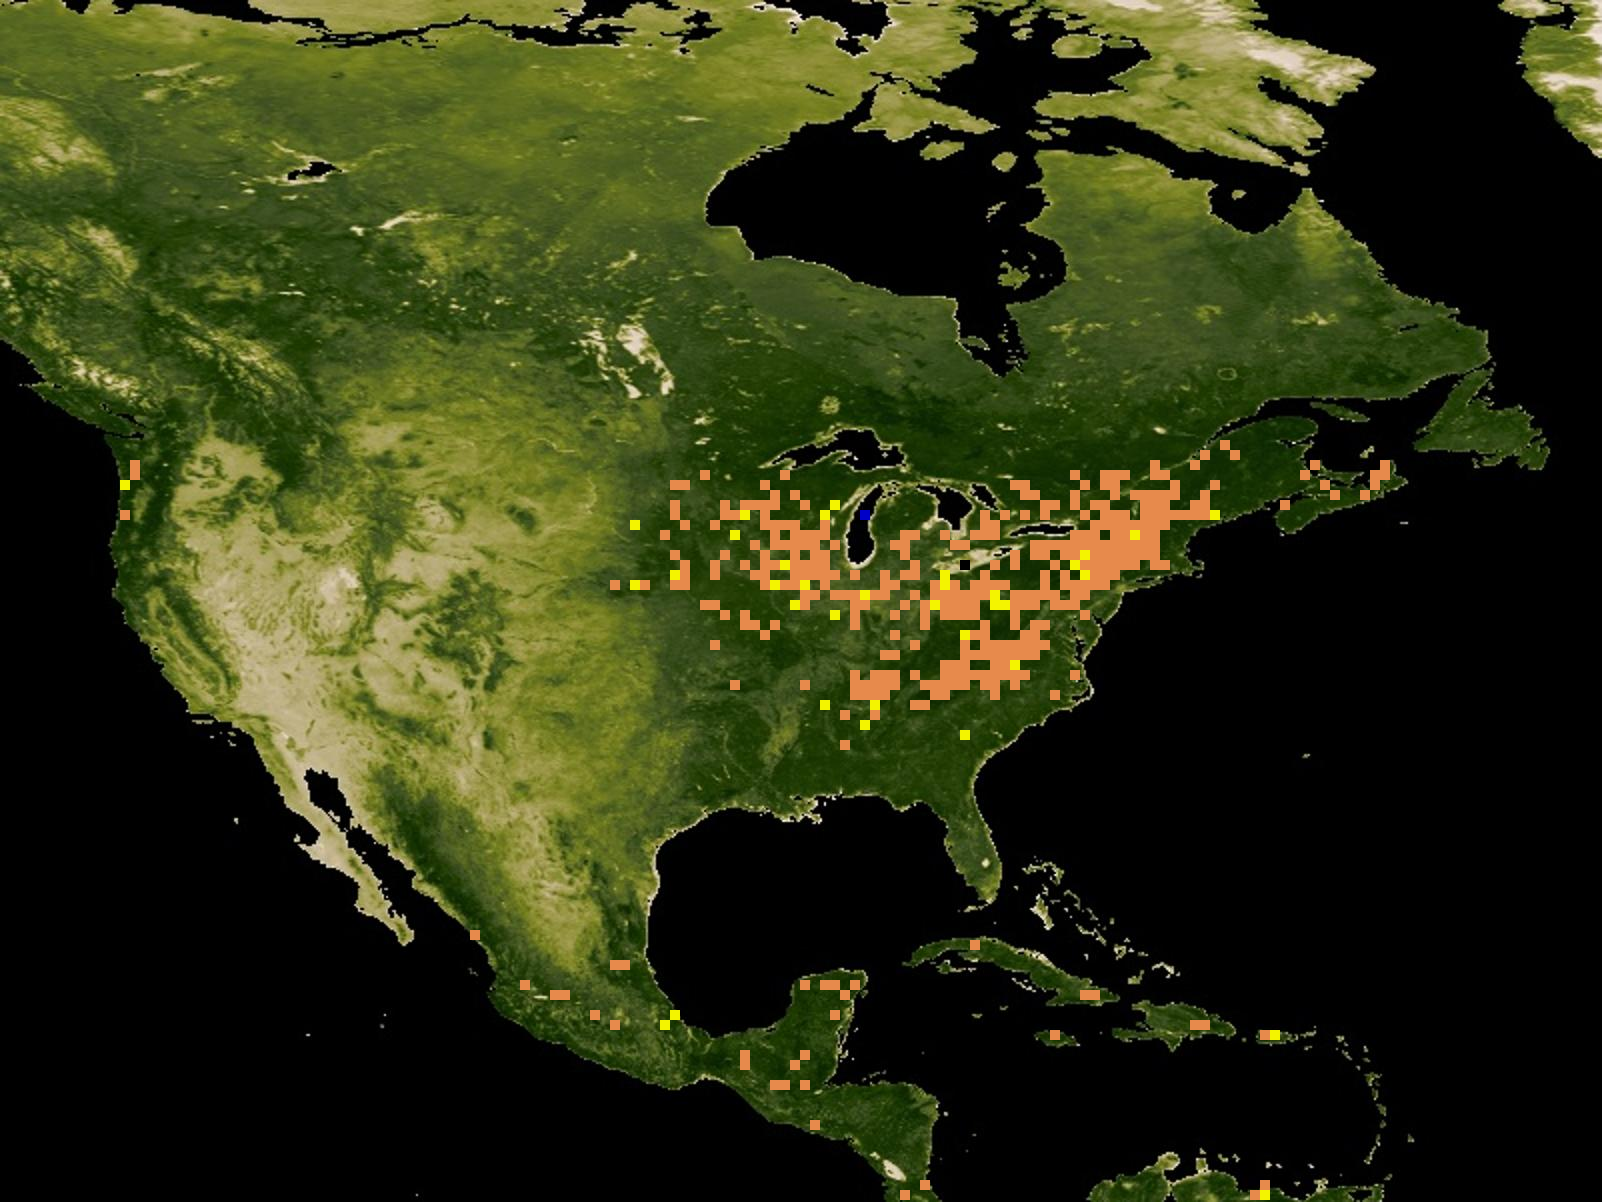
\includegraphics[width=0.10\textwidth]{map/83.png} &
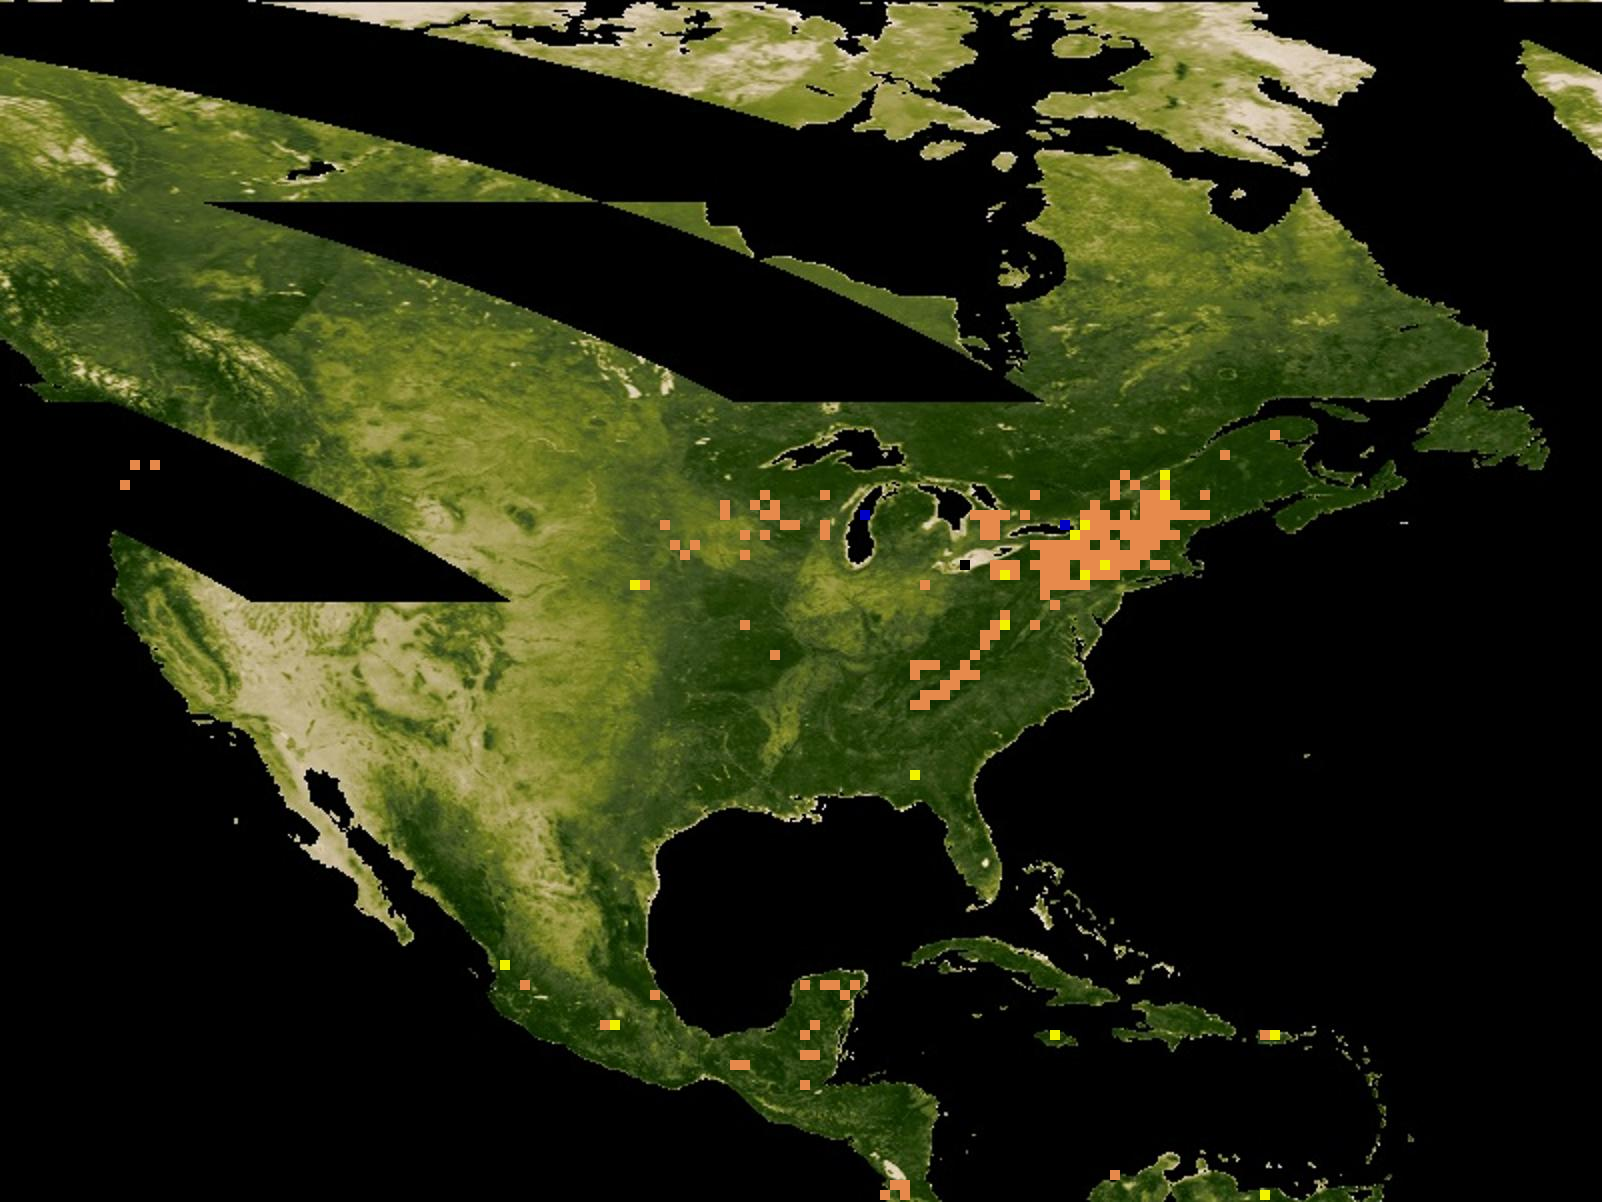
\includegraphics[width=0.10\textwidth]{map/84.png} &
%\includegraphics[width=0.5\textwidth,height=1.4in,clip,trim=0 0.5in 0in 0.6in]{plots/chicago_noaa_vs_prediction_prev_3.png} 
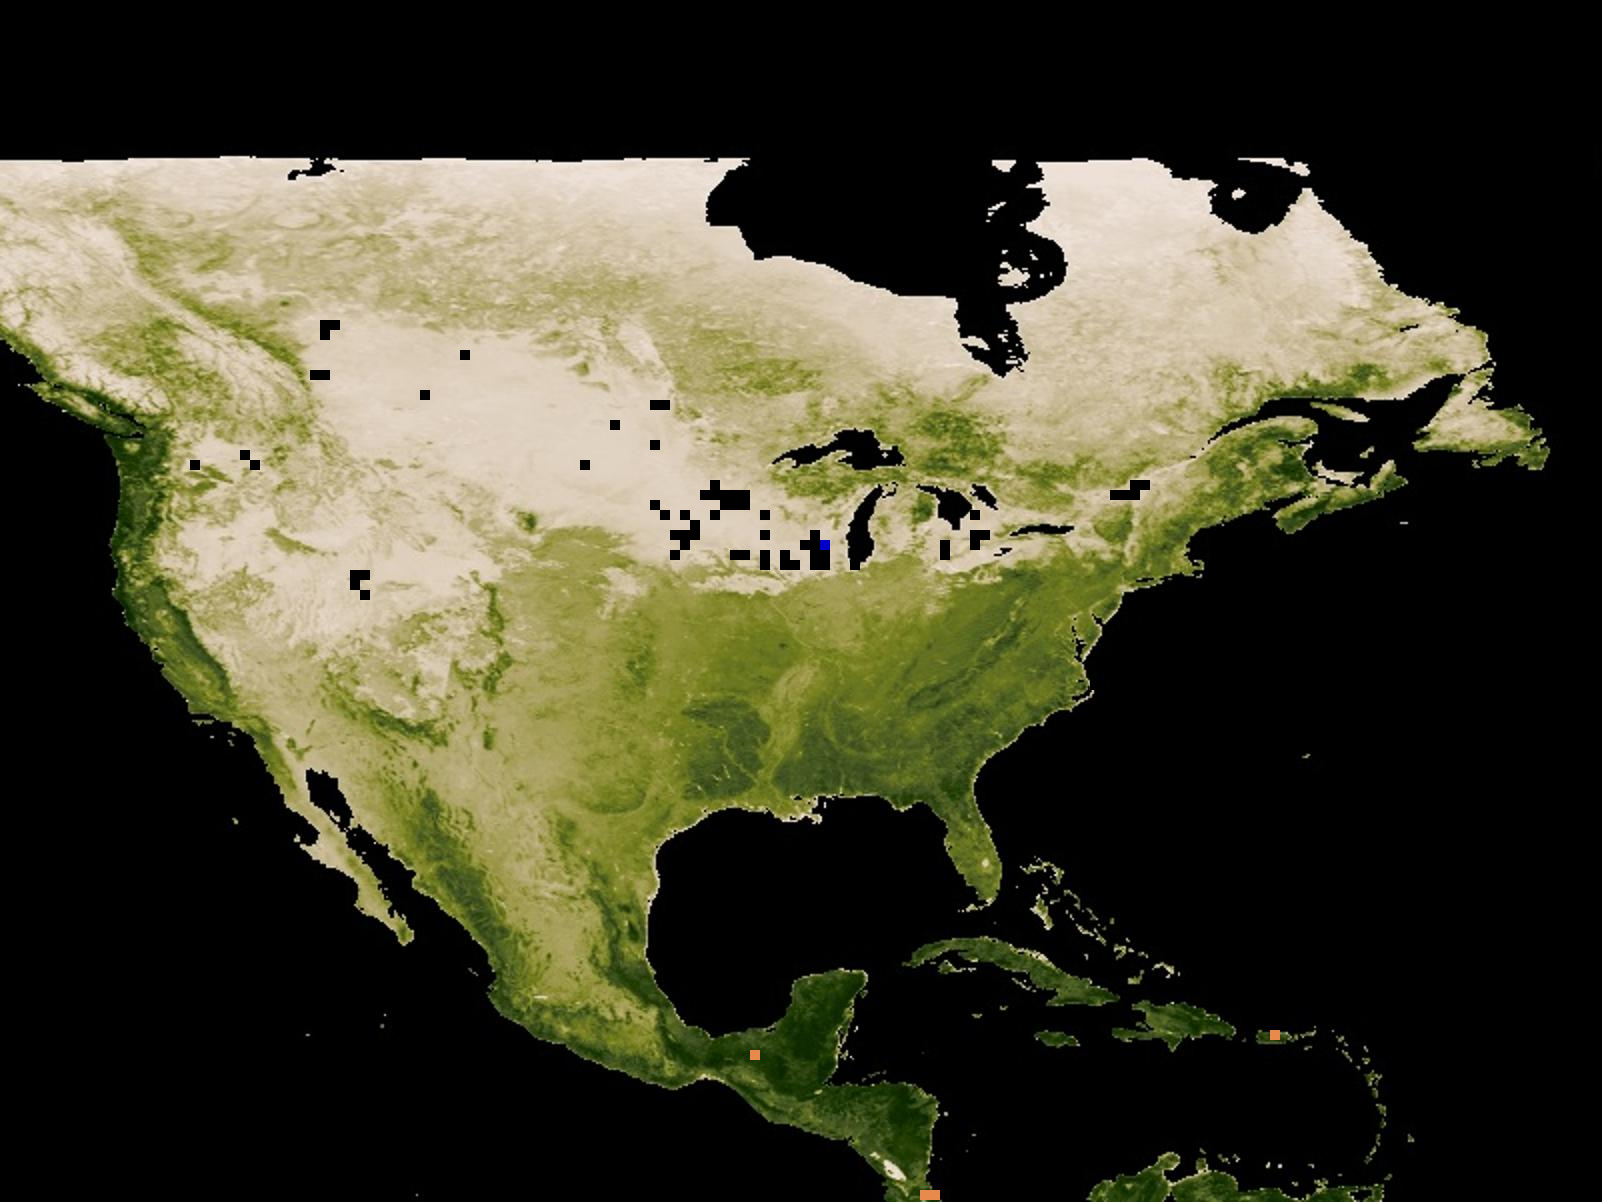
\includegraphics[width=0.10\textwidth]{map/91.png}  \\
Aug, 13th&Aug, 29th&Sep, 14th&Dec 19th\\
\\
\end{tabular}
\end{center}
%}}
\vspace{-24pt}
\caption{%On two 16-days time period, end of August on the left and during Christmas on the right, we show the confusion matrix map here. Orange bins are true positive; yellow bins are false negative; blue bins are false positive; and black bins are true negative.
We use prediction results to recreate vegetation coverage maps for each 16-days period. There are 8 maps picked in 2010. The dates under each map are the starting date of each 16-days period.
Orange bins represent true positive; blue bins are false positives; yellow bins are true negatives and black bins are false negatives. }
\label{fig:map}
\vspace{-12pt}
\end{figure}